\hspace{0.5cm} In their paper \cite{bib11}, Li et al describe that in order to perform UST, the models required are five pairs of encoder-decoders based on the VGG-19 architecture. They work as a pipeline where each encoder-decoder pair is a pipeline level (see Fig.~\ref{fig:full-pipeline}). In each such pair, the encoder serve as feature extractor while the decoder does the inverse operation, reconstructs the image from the extracted features.\\
We based our solution on the implementation of VGG-19 \cite{bib20} in \texttt{torchvision.models}. It is trained for image classification on the ImageNet dataset (Deng et al.) \cite{bib21}. The model is available with pretrained weights. Its CNN feature extractor has the following architecture: 
\begin{gather*}
[64, 64, MP, 128, 128, MP, 256, 256, 256, 256, MP, 512, 512, 512, 512, MP, 512, 512, 512, 512, MP]
\end{gather*}

\subsubsection{Encoders}
Any numeric $d$ entry indicates a 2D-convolution layer with $d$ output channels, and MP entries indicate MaxPool layers. In order to build the five encoders, we load the \texttt{torchvision.models} VGG-19 pretrained model and trim it in the following way:
\begin{itemize}
	\item Encoder-1: [64]
	\item Encoder-2: [64, 64, MP, 128]
	\item Encoder-3: [64, 64, MP, 128, MP, 256]
	\item Encoder-4: [64, 64, MP, 128, MP, 256, 256, 256, 256, MP, 512]
	\item Encoder-5: [64, 64, MP, 128, MP, 256, 256, 256, 256, MP, 512, 512, 512, 512, MP, 512]
\end{itemize}
The encoders are initialized with pretrained weights and thus the project does not include encoder training. For next sections, denote Encoder-$j$ as $E_j$.

\subsubsection{Decoders}
The architecture of the decoders is generally inverse to that of the encoders, in order to achieve image-reconstruction. We defined five decoder \textit{blocks} the following way:
\begin{itemize}
	\item Decoder-Block-1: (64)[3]
	\item Decoder-Block-2: (128)[64, US, 64]
	\item Decoder-Block-3: (256)[128, US, 128]
	\item Decoder-Block-4: (512)[256, US, 256, 256, 256]
	\item Decoder-Block-5: (512)[512, US, 512, 512, 512]
\end{itemize}
The number in parenthesis in each row stands for the number of input channels for the block, and every US entry stands for an Up Sampling layer. Let's denote Decoder-Block-$j$ by $B_j$. Each decoder then is built as such:
\begin{equation}\label{eq:decoder}
D_j(x) = B_1 \circ \dots \circ B_j (x)
\end{equation}

Decoder training was done with two steps: Decoder-Block sequential training, followed by Fine-Tune phase.
\begin{itemize}
	\item \textbf{Decoder-Block sequential training}: Initially $B_1$ was trained to reconstruct images encoded by Encoder-1. Afterwards, each $B_j, j>1$ was trained once all $j-1,\dots,1$ had finished training to some reasonable degree. In training $B_j$, the reconstruction result for image $x$ was calculated by:
	\begin{gather*}
	\hat{x} = B_1 \circ \dots \circ B_{j-1} \circ B_j \circ E_j (x)
	\end{gather*}
	In this calculation all functions except $B_j$ are fixed. Since $B_{j-1}, \dots, B_1$ are already pretrained to some degree when training $B_j$, then $B_j$ learns to transform $E_j$'s output to $D_{j-1}$ input.
	
	\item \textbf{Fine-Tune Phase}: Each decoder $D_j$ is built according to Equation~\ref*{eq:decoder} with the pretrained blocks acquired in the previous step. With none of the blocks frozen, the entire $D_j$ is now trained for image reconstruction against $E_j$ and ultimately is saved as a decoder (and not as a bundle of blocks).
\end{itemize}

Throughout this section, the loss function for training the models is:
\begin{equation}
L = MSE(I_o-I_i) + \lambda \cdot MSE(\Phi(I_o)-\Phi(I_i))
\end{equation}
It is derived from Equation 1 at \cite{bib11}, with the difference that we use $MSE$ where Li et al use $L2 -loss$. We chose to use $MSE$ since different encoders $\Phi$ output different dimensions, causing the $L2$ loss to be  somewhat not as normalized as the $MSE$. For example, an input image $I_i$ of dimensions [3,1024,1024] would have features $f_4=E_4(I_i)$ of dimension [512, 128, 128] for $D_4$ training, 8,388,608 total entries, whereas it would have $f_5=E_5(I_i)$ of dimension [512, 64, 64] for $D_5$ training, 2,097,152 total entries. In this example, the dimension difference causes the feature loss to be much more important in $D_4$ training than in $D_5$ under $L2$, while we believe it shouldn't.

$\lambda$ was set to $1.0$ during training as advised by Li et al in their paper \cite{bib11}.

\textcolor{red}{TODO}: when training we encountered two problems: "boxy" artifacts in $D_4, D_5$ and border artifacts in $D_1$. to mitigate these problems we set the UpSampling in blocks 4,5 to "bilinear" whereas in 1,2,3 is "nearest", and in $D_1$ only, we set the padding method of $B_1$ from zero-padding to replicate padding.

\textcolor{red}{TODO}: discuss why we chose to train the models sequentially - smaller models converge faster, we wanted to use this to obtain a "good" starting point for the fine tuning.

\textcolor{red}{TODO}: COCO Dataset

\begin{figure}[h!]
	\centering
	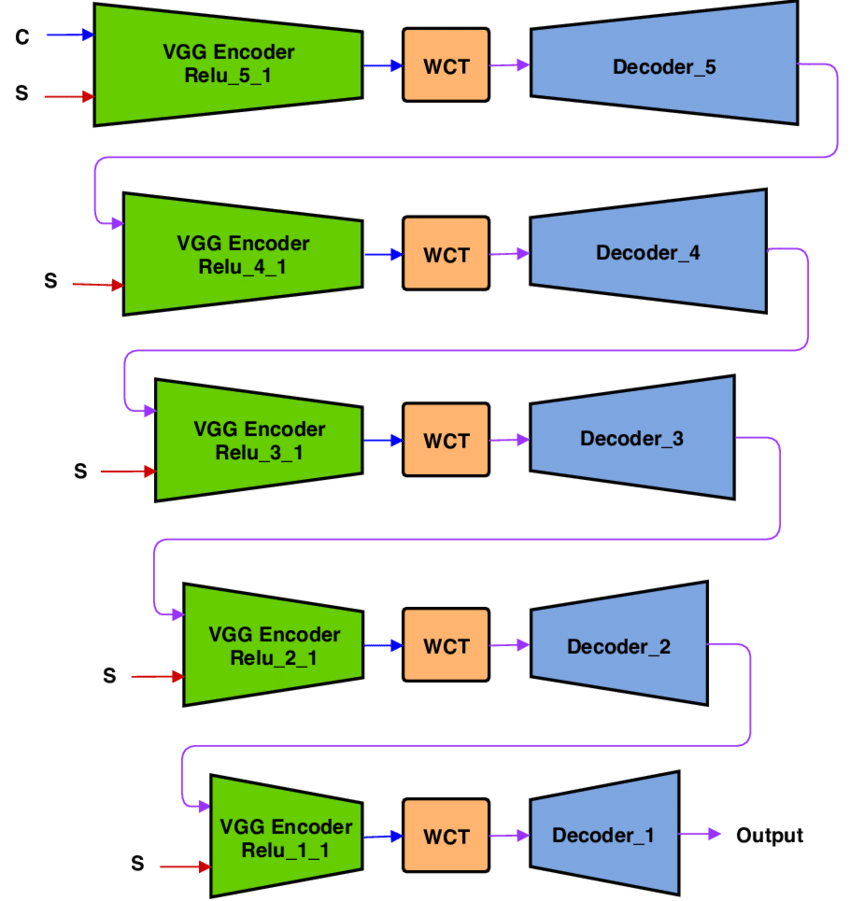
\includegraphics[width=0.5\linewidth]{UST_arc_mlt_level_pipeline.png}
	\caption{Universal Style Transfer architecture with the whole multi level pipeline. Each level of stylization consists of single encoder-WCT-decoder network with different decreasing number of VGG layers. C and S are content and style images, respectively.
	}
	\label{fig:full-pipeline}
\end{figure}